%%%%%%%%%%%%%%%%%%%%%%%%%%%%%%%%%%%%%%%%%%%%%%%%%%%%%%%%%%%
%%%%%%%%%%%%%%%%%%%%%%%%%%%%%%%%%%%%%%%%%%%%%%%%%%%%%%%%%%%
\subsection{EMMA}
%%%%%%%%%%%%%%%%%%%%%%%%%%%%%%%%%%%%%%%%%%%%%%%%%%%%%%%%%%%%%%%%%%%%%%%%%%%%%%%%%%%%%%%%5
\subsubsection{what is best}
\begin{align}
%    G    & = -3.7 + 0.18 * TCal +  8.1 * max(0,6-layr)\\
%    \rho & = -0.78 + 0.0024 * TCal + 0.13 * max(0,6-layr)
    G &=      -19 + 0.28 * TCal  - 0.022 * layr*TCal  +  0.16 * h(layr-6)*TDOC \\
    \rho &=  -0.87 + 0.0047 * TCal  - 0.00036 * layr*TCal  +  0.0024 * h(layr-6)*TDOC \\
    \lambda &=  6.8 - 0.014 * TCal  + 0.0018 * layr*TCal  + 0.0060 * h(layr-6)*TDOC \\
    v_{cal} &= 29 - 0.052 * TCal  + 0.0011 * layr*TCal  -  0.011 * h(layr-6)*TDOC 
\end{align}
what was the best result? For each particle there is best and global best. 
https://stackoverflow.com/questions/30228281/gnuplot-parallel-coordinates-axes-plot-key-annotation

%%%%%%%%%%%%%%%%%%%%%%%%%%%%%%%%%%%%%%%%%%%%%%%%%%%%%%%%%%%%%%%%%%%%%%%%%%%%%%%%%%%%%%%%5
\subsubsection{how did evolve over time?}

\begin{table}[h]
	\centering
    \caption{Global best per generation}
	\label{tab:emma_gen}
	\begin{tabular}{cccccccc}
        \hline\hline
    generation  &enr &conc &layr &vDOC &TDOC &vCal &TCal\\
        \hline
     1   &1       &2    &4   &10   &40  &120  &300\\
     2   &5       &2    &6   &10   &40  &120  &300\\
     3   &2947    &4    &6   &16   &80 &1080  &300\\
     4   &2405    &2    &6   &10   &40 &1080  &300\\
     5   &13      &2   &10   &10   &40  &120  &300\\
    \hline\hline
	\end{tabular}
\end{table}

\begin{figure}
    \centering
    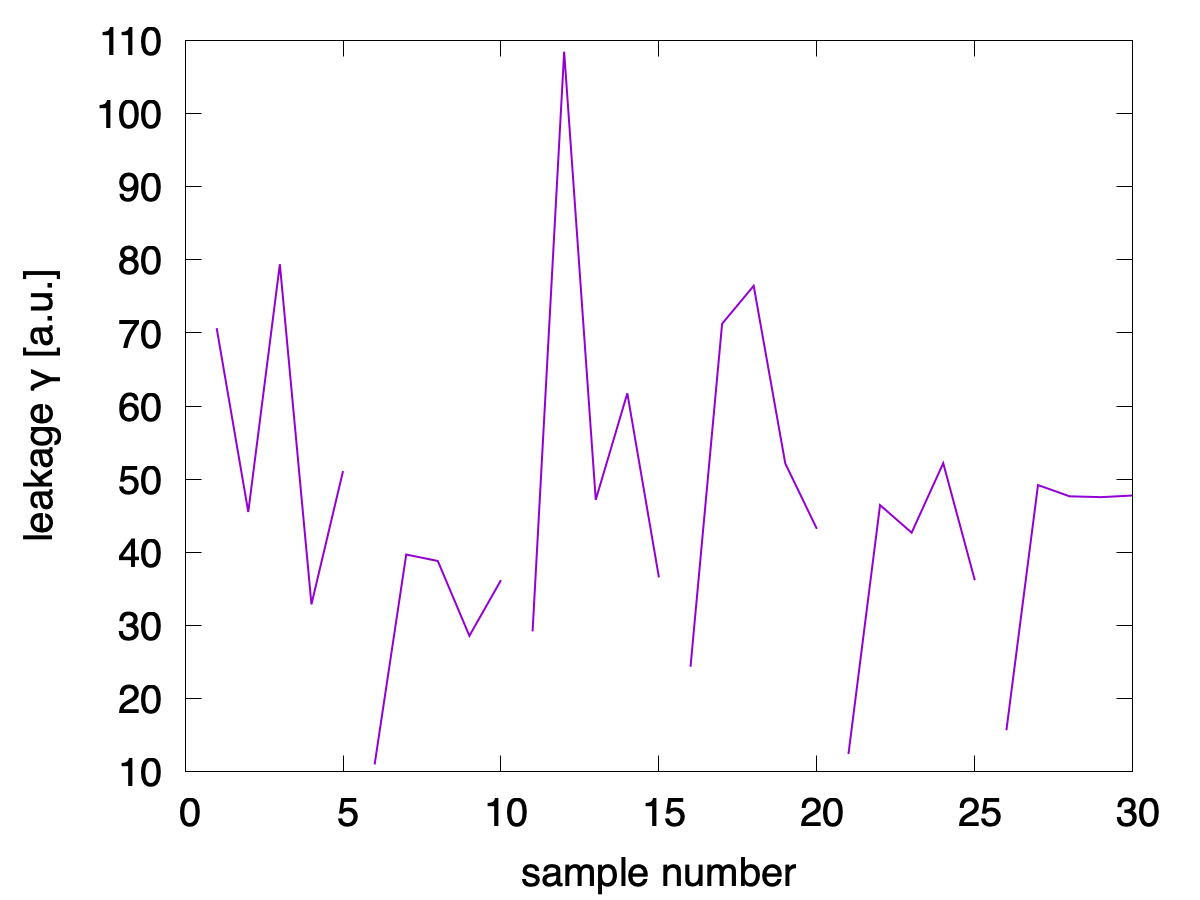
\includegraphics[width=.6\textwidth]{Pics/stats/G-t.png}
    \caption{conductivity G [a.u.] against sample number (is this even correct?)}
    \label{fig:G-t}
\end{figure}

\td{TODO: check if the sorted correctly? Make generation graph with boxplot }
    \td{TODO: visualize} how the population moved across the space (with parallel coordinates? or see page 121)
        \url{https://stackoverflow.com/questions/30228281/gnuplot-parallel-coordinates-axes-plot-key-annotation}

%%%%%%%%%%%%%%%%%%%%%%%%%%%%%%%%%%%%%%%%%%%%%%%%%%%%%%%%%%%%%%%%%%%%%%%%%%%%%%%%%%%%%%%%5
\subsubsection{how did model selection influence results}
\begin{itemize}
    \item MARS chooses same set from independent variables for predicting all dependent variables. 
    \item flaws of MARS: all functions are dependent on same indep vars
    \item Every output var is independent of each other, so $v_{cal}$ can act as test 
heating rate was one of the dependent variables with the intention of minimizing the variable. 
It can also be used as test to see how well the EMMA performes (or rather, more precisely MARS)
It doesn't influence the fit for the other splines, but it influences the choice of samples therefore it might have slowed down the process
Overall there were too many variables involved for such a small dataset
        that means that adding dependent variables influences \td{previous variables}
\end{itemize}

%%%%%%%%%%%%%%%%%%%%%%%%%%%%%%%%%%%%%%%%%%%%%%%%%%%%%%%%%%%%%%%%%%%%%%%%%%%%%%%%%%%%%%%%5
\subsubsection{analyse data with other methods post optimization}
\begin{itemize}
    \item ANOVA (influence of TCal) \texttt{Code/Statistics/sub/anova.R}
    \item lin regression (influence of conc) \texttt{Code/Statistics/sub/linreg.py}
    \item grid search 
    \item KRR (???)
    \item SVM (???)
\end{itemize}

and cite something pro forma \cite{ncbi1butanol}
\td{plot the predicted data for variables which should be excluded (Tcal, Vcal,Conc, layers)}
